% orig.tex -- Sections 1--10 of the Checkpoint 2 report (BTP_Checkpoint2.pdf, 13 pp., 2026-09-18),
% re-typeset verbatim from the compiled PDF. Domain: orig.
% Look of the original: \documentclass[11pt]{article}, US letter, 1in margins (geometry
% margin=1in), Computer Modern, floats placed with [H] (float package) except Table 6.
% Only layout defects were changed: Table 1 (overflowed the right page edge) is re-set with
% tabularx and its truncated cells completed from the text still present in the original PDF
% (cross-checked with spider_web_htn/operators.py); Algorithm 5 line 5 (ran into the right
% margin) is wrapped. Everything else -- including errors -- is as printed.
% Hard-coded internal references are \ref's, except those that are wrong/ambiguous in the
% original ("Line 15", "\S5", "\S1", "Table 1's geometry", sections of external documents),
% which are kept literally.
\providecommand{\origstick}[2]{\mathrm{stick}_{#1}^{\mathrm{#2}}}
\providecommand{\origpath}[1]{\mathrm{path}_{\mathrm{#1}}}

\section{Preliminaries and Notation}
\label{sec:orig-prelim}

Let the web-construction problem be defined by a state space $\mathcal{S}$, a set of primitive operators $\mathcal{O}$, and a set of compound tasks $\mathcal{T}$. A state $s \in \mathcal{S}$ is a tuple
\[
  s = \bigl\langle\, p,\ N,\ E,\ c_1, \dots, c_k \,\bigr\rangle,
\]
where $p$ is the spider's current position, $N$ is the set of named structural/anchor nodes discovered so far, $E$ is the set of laid threads (each an edge labelled with a thread type, e.g.\ \textit{bridge}, \textit{dragline}, \textit{proto-radius}, \textit{frame}, \textit{radius}, \textit{auxiliary spiral}, \textit{capture spiral}), and $c_1, \dots, c_k$ are scalar/boolean progress counters (e.g.\ number of proto-radii laid, number of frame threads completed, cumulative energy expended).

A \textit{primitive operator} $o \in \mathcal{O}$ is a partial function $o : \mathcal{S} \rightharpoonup \mathcal{S}$ applicable only when its preconditions hold in $s$; applying it yields a successor state $s' = o(s)$ (or $\bot$ on precondition failure). A \textit{compound task} $t \in \mathcal{T}$ is decomposed by one or more \textit{methods} $m : \mathcal{S} \rightharpoonup (\mathcal{T} \cup \mathcal{O})^*$, each returning an ordered list of subtasks, or $\bot$ if inapplicable.

\section{Generic HTN Forward-Search Planning Procedure}
\label{sec:orig-htn}

The underlying planner (GTPyhop-style total-order forward decomposition with chronological backtracking)\cpnote{The planner as configured for the runs reported here does not backtrack. The installed GTPyhop~1.9.7 defaults to an iterative greedy strategy that commits to the first applicable method, and no run in the repository selects another strategy (Section~\ref{sec:recovery-strategy}). Algorithm~\ref{alg:orig-findplan} is a correct statement of depth-first search with chronological backtracking, but it is not the search that produced these plans. Re-running the anchor-removal sweep with explicit backtracking gave the same outcome in all 9{,}000 trials (Section~\ref{sec:core-config}).} is domain-independent and is stated once here; Section~\ref{sec:orig-domain} instantiates it with the biologically-derived task/method library.

\begin{algorithm}[H]
\algrenewcommand\algorithmicrequire{\textbf{Input:}}
\algrenewcommand\algorithmicensure{\textbf{Output:}}
\caption{\textsc{FindPlan} --- Total-order HTN forward decomposition}
\label{alg:orig-findplan}
\begin{algorithmic}[1]
\Require initial state $s_0 \in \mathcal{S}$, initial task list $T_0 = [t_1, \dots, t_n]$
\Ensure a primitive action sequence $\pi$ achieving $T_0$ from $s_0$, or \textsc{Fail}
\Function{FindPlan}{$s, T$}
  \If{$T = \emptyset$}
    \State \Return $[\,]$ \Comment{empty plan: base case}
  \EndIf
  \State $t \gets \mathrm{head}(T)$; \quad $T' \gets \mathrm{tail}(T)$
  \If{$t \in \mathcal{O}$} \Comment{$t$ is primitive}
    \State $s_1 \gets t(s)$
    \If{$s_1 = \bot$}
      \State \Return \textsc{Fail}
    \EndIf
    \State $\pi' \gets{}$\Call{FindPlan}{$s_1, T'$}
    \If{$\pi' \neq \textsc{Fail}$}
      \State \Return $[t] \,\|\, \pi'$
    \Else
      \State \Return \textsc{Fail}
    \EndIf
  \Else \Comment{$t$ is compound}
    \For{each method $m$ registered for $t$, \textbf{in declared order}}
      \State \textit{subtasks} $\gets m(s)$
      \If{\textit{subtasks} $\neq \bot$} \Comment{method applicable}
        \State $\pi' \gets{}$\Call{FindPlan}{$s,\ \textit{subtasks} \,\|\, T'$}
        \If{$\pi' \neq \textsc{Fail}$}
          \State \Return $\pi'$ \Comment{success --- no further backtracking}
        \EndIf \Comment{else: implicit backtrack --- try next method $m$}
      \EndIf
    \EndFor
    \State \Return \textsc{Fail} \Comment{all methods for $t$ exhausted}
  \EndIf
\EndFunction
\end{algorithmic}
\end{algorithm}

Line 15 is the point\cpnote{``Line 15'' is as printed in Checkpoint~2; the loop over methods is lines 18--26 of Algorithm~\ref{alg:orig-findplan}.} at which Zschokke's observed \textit{behavioural variability} is realised computationally: whenever a compound task has more than one registered method, the planner commits to the first applicable one and backtracks to the next only upon downstream failure, so any of several biologically valid strategies may appear in the final plan.

\section{Domain Task Decomposition}
\label{sec:orig-domain}

\subsection{Top-level task}
\label{sec:orig-toplevel}

\begin{algorithm}[H]
\caption{Method for \textsc{Build-Web}}
\label{alg:orig-buildweb}
\begin{algorithmic}[1]
\Function{Build-Web}{$s$}
  \If{$s.$\textit{web\_complete}}
    \State \Return $[\,]$
  \EndIf
  \State \Return $[\,$\textsc{Explore-And-Bridge}, \textsc{Establish-Proto-Hub},\newline
    \hspace*{90pt}\textsc{Build-Remaining-Web}, \textsc{Finalise-Web}$\,]$
\EndFunction
\end{algorithmic}
\end{algorithm}

\subsection{Early stage I --- exploration and bridging (single method)}
\label{sec:orig-explore}

Zschokke: the spider bridges the gap between supports by attaching a dragline at one support and walking a detour along the base of the structure, then establishes the highest possible thread.

\begin{algorithm}[H]
\caption{Method for \textsc{Explore-And-Bridge}}
\label{alg:orig-explore}
\begin{algorithmic}[1]
\Function{Explore-And-Bridge}{$s$}
  \If{$s.$\textit{bridge\_established}}
    \State \Return $[\,]$
  \EndIf
  \State \Return $\bigl[$\,\Call{Attach-Dragline}{$\origstick{R}{top}$}, \Call{Walk}{$\origstick{R}{top}, \origstick{R}{bot}$},\newline
    \hspace*{85.8pt}\Call{Walk}{$\origstick{R}{bot}, \origpath{bot}$}, \Call{Walk}{$\origpath{bot}, \origstick{L}{bot}$},\newline
    \hspace*{85.8pt}\Call{Walk}{$\origstick{L}{bot}, \origstick{L}{mid}$}, \Call{Lay-Thread}{$\origstick{L}{mid}, \origstick{R}{top}, \textit{bridge}$},\newline
    \hspace*{85.8pt}\textsc{Establish-High-Thread}\,$\bigr]$
\EndFunction
\end{algorithmic}
\end{algorithm}

\subsection{Early stage II --- proto-hub establishment (variable, backtracking)}
\label{sec:orig-protohub}

This is the central behavioural finding formalised by the model: Zschokke documented \textit{three} distinct ways a spider reaches the supporting structure while laying a proto-radius (walking along existing threads, dropping vertically on the dragline, or the ``Tarzan'' swing method). All three are registered as alternative methods for the same task, so Algorithm~\ref{alg:orig-findplan} non-deterministically explores them, backtracking on failure\cpnote{In every plan generated in the repository the \textit{via-walk} method is the one selected. The drop and Tarzan variants are encoded in the method library but have never occurred in a plan: we counted no \textsc{Drop-Down} or \textsc{Swing-Tarzan} action in 3{,}819 successful plans at commit \texttt{39b89f3} or in 1{,}137 at \texttt{61d18d8} (Section~\ref{sec:core-config}).} --- this is what reproduces the empirically observed opportunism.

\begin{algorithm}[H]
\caption{Methods for \textsc{Establish-Proto-Hub} (three biologically motivated alternatives, tried in order with backtracking)}
\label{alg:orig-protohub}
\begin{algorithmic}[1]
\Function{Establish-Proto-Hub}{$s$} \Comment{base case}
  \If{$s.$\textit{proto\_hub\_exists}}
    \State \Return $[\,]$
  \EndIf
  \State \Return $\bot$ \Comment{fall through to variant methods below}
\EndFunction
\Statex
\Function{Establish-Proto-Hub-Via-Walk}{$s$} \Comment{variant 1 of 3}
  \State $a \gets \mathrm{Anchors}_{\mathrm{walk}}[\,s.\textit{proto\_radii\_count} \bmod 8\,]$
  \State \textit{subtasks} $\gets [\,$\Call{Anchor}{hub}, \Call{Lay-Thread}{$\text{hub}, a, \textit{dragline}$},\newline
    \hspace*{108.5pt}\Call{Reel-Up}{$a, \text{hub}$}, \Call{Insert-Radius}{$a, \text{hub}$}$\,]$
  \If{$s.$\textit{proto\_radii\_count} $\geq 3$}
    \State \textbf{append} \Call{Mark-Proto-Hub}{hub} to \textit{subtasks}
  \Else
    \State \textbf{append} \textsc{Establish-Proto-Hub} to \textit{subtasks} \Comment{recurse}
  \EndIf
  \State \Return \textit{subtasks}
\EndFunction
\Statex
\Function{Establish-Proto-Hub-Via-Drop}{$s$} \Comment{variant 2 of 3}
  \State $a \gets \mathrm{Anchors}_{\mathrm{drop}}[\,s.\textit{proto\_radii\_count} \bmod 6\,]$
  \State \textit{subtasks} $\gets [\,$\Call{Anchor}{hub}, \Call{Drop-Down}{$\text{hub}, a$},\newline
    \hspace*{108.5pt}\Call{Reel-Up}{$a, \text{hub}$}, \Call{Insert-Radius}{$a, \text{hub}$}$\,]$
  \State \textit{(append \textsc{Mark-Proto-Hub} or recurse, as above)}
  \State \Return \textit{subtasks}
\EndFunction
\Statex
\Function{Establish-Proto-Hub-Via-Tarzan}{$s$} \Comment{variant 3 of 3}
  \State $a \gets \mathrm{Anchors}_{\mathrm{tarzan}}[\,s.\textit{proto\_radii\_count} \bmod 6\,]$
  \State \textit{subtasks} $\gets [\,$\Call{Anchor}{hub}, \Call{Swing-Tarzan}{$\text{hub}, a$},\newline
    \hspace*{108.5pt}\Call{Reel-Up}{$a, \text{hub}$}, \Call{Insert-Radius}{$a, \text{hub}$}$\,]$
  \State \textit{(append \textsc{Mark-Proto-Hub} or recurse, as above)}
  \State \Return \textit{subtasks}
\EndFunction
\end{algorithmic}
\end{algorithm}

A proto-hub is confirmed once four proto-radii have converged on the same point:
\[
  \textsc{Mark-Proto-Hub}(\text{hub}) \text{ applicable} \iff s.\textit{proto\_radii\_count} \geq 4.
\]

\subsection{Later stages --- stereotyped, single-method decomposition}
\label{sec:orig-later}

Once the proto-hub exists, construction becomes a fixed procedural sequence (frame $\to$ radii $\to$ auxiliary spiral $\to$ capture spiral), matching Zschokke's description of a ``rigid pattern'' in this phase.

% Layout fix: in the original, line 5 of this algorithm ran 22pt into the right margin; it is
% wrapped here after "Build-Auxiliary-Spiral,".
\begin{algorithm}[H]
\caption{Method for \textsc{Build-Remaining-Web}}
\label{alg:orig-remaining}
\begin{algorithmic}[1]
\Function{Build-Remaining-Web}{$s$}
  \If{$\neg\, s.$\textit{proto\_hub\_exists}}
    \State \Return $\bot$
  \EndIf
  \State \Return $[\,$\textsc{Build-Frame}, \textsc{Build-Radii}, \textsc{Build-Auxiliary-Spiral},\newline
    \hspace*{\algorithmicindent}\phantom{\textbf{return} $[\,$}\textsc{Build-Capture-Spiral}$\,]$
\EndFunction
\end{algorithmic}
\end{algorithm}

\begin{algorithm}[H]
\caption{Method for \textsc{Build-Frame} --- top frame first, then left, bottom, right}
\label{alg:orig-frame}
\begin{algorithmic}[1]
\Function{Build-Frame}{$s$}
  \If{$s.$\textit{frame\_count} $\geq 4$}
    \State \Return $[\,]$
  \EndIf
  \State $h \gets s.$\textit{proto\_hub\_pos}
  \State $F \gets \bigl[\,(\origstick{L}{top}, \origstick{R}{top}),\ (\origstick{L}{top}, a_{LL}),\ (a_{LL}, a_{RL}),\ (a_{RL}, \origstick{R}{top})\,\bigr]$ \Comment{top, left, bottom, right}
  \State \textit{subtasks} $\gets [\,]$
  \For{$(n_1, n_2) \in F[\,s.\textit{frame\_count}:\,]$}
    \State \textbf{append} \Call{Walk}{$h, n_1$}, \Call{Lay-Frame-Thread}{$n_1, n_2$}, \Call{Walk}{$n_2, h$} to \textit{subtasks}
  \EndFor
  \State \Return \textit{subtasks}
\EndFunction
\end{algorithmic}
\end{algorithm}

\begin{algorithm}[H]
\caption{Method for \textsc{Build-Radii} --- circle hub, fill gaps until 8 radii placed}
\label{alg:orig-radii}
\begin{algorithmic}[1]
\Function{Build-Radii}{$s$}
  \If{$s.$\textit{radii\_count} $\geq 8$}
    \State \Return $[\,]$
  \EndIf
  \State $h \gets s.$\textit{proto\_hub\_pos}; \quad $R \gets \mathrm{Anchors}_{\mathrm{radii}}[\,s.\textit{radii\_count}:\,]$
  \State \textit{subtasks} $\gets [\,]$
  \For{$a \in R$}
    \State \textbf{append} \Call{Walk}{$h, h$}, \Call{Lay-Radius}{$h, a$}, \Call{Walk}{$a, h$} to \textit{subtasks} \Comment{circle hub $\to$ place radius $\to$ return}
  \EndFor
  \State \Return \textit{subtasks}
\EndFunction
\end{algorithmic}
\end{algorithm}

\begin{algorithm}[H]
\caption{Method for \textsc{Build-Auxiliary-Spiral} / \textsc{Build-Capture-Spiral} --- Archimedean spiral traversal}
\label{alg:orig-spiral}
\begin{algorithmic}[1]
\Function{Build-Spiral}{$s$, \textit{direction}, $t_{\mathrm{start}}$, $t_{\mathrm{end}}$, \textit{turns}, \textit{type}} \Comment{\textit{direction} = outward (auxiliary, $t_s{=}0.20 \to t_e{=}0.80$) or inward (capture, $t_s{=}0.85 \to t_e{=}0.20$)}
  \State $h \gets s.$\textit{proto\_hub\_pos}; \quad $A \gets \mathrm{Anchors}_{\mathrm{radii}}$
  \State $N \gets \textit{turns} \times |A|$
  \State \textit{prev} $\gets h$; \quad \textit{subtasks} $\gets [\,]$
  \For{$i \gets 0$ \textbf{to} $N - 1$}
    \State \textit{frac} $\gets t_{\mathrm{start}} + i \cdot \dfrac{t_{\mathrm{end}} - t_{\mathrm{start}}}{N - 1}$
    \State \textit{curr} $\gets$ \Call{GetRadiusNode}{$A[\,i \bmod |A|\,]$, \textit{frac}}
    \State \textbf{append} \Call{Build-Spiral-Segment}{\textit{prev}, \textit{curr}, \textit{type}} to \textit{subtasks}
    \State \textit{prev} $\gets$ \textit{curr}
  \EndFor
  \State \textbf{append} \Call{Walk}{\textit{prev}$, h$}, \Call{Mark-Spiral-Done}{\textit{type}} to \textit{subtasks}
  \State \Return \textit{subtasks}
\EndFunction
\end{algorithmic}
\end{algorithm}

\subsection{Finalisation}
\label{sec:orig-finalisation}

\begin{algorithm}[H]
\caption{Method for \textsc{Finalise-Web}}
\label{alg:orig-finalise}
\begin{algorithmic}[1]
\Function{Finalise-Web}{$s$}
  \If{$s.$\textit{web\_complete}}
    \State \Return $[\,]$
  \EndIf
  \State \Return $[\,$\textsc{Mark-Web-Complete}$\,]$
\EndFunction
\end{algorithmic}
\end{algorithm}

\section{Primitive Operators}
\label{sec:orig-operators}

Each primitive operator $o \in \mathcal{O}$ is a guarded state transition. Table~\ref{tab:orig-operators} summarises preconditions and effects;\cpnote{The right-hand column of this table ran off the page in the Checkpoint~2 PDF and is restored here in full. In the code, \textsc{Lay-Frame-Thread} and \textsc{Lay-Radius} also add $d(u,v)$ to the energy total (\texttt{spider\_web\_htn/operators.py}); the table omits that effect for these two rows.} $d(n_1, n_2)$ denotes Euclidean distance between nodes, used as the locomotory cost (Section~\ref{sec:orig-energy}).

% Layout fix: in the original this table was a plain l/l/l tabular that ran off the right edge
% of the page, cutting the Effect column. Re-set to the text width; the cut-off cells
% (Lay-Thread, Drop-Down, Swing-Tarzan, Insert-Radius, Lay-Frame-Thread, Lay-Radius,
% Build-Spiral-Segment) are completed with the text that is still present, outside the page,
% in the original PDF (checked against spider_web_htn/operators.py).
\begin{table}[H]
\centering
{\footnotesize
\setlength{\tabcolsep}{4pt}
\begin{tabularx}{\linewidth}{@{}l>{\raggedright\arraybackslash}p{3.5cm}>{\raggedright\arraybackslash}X@{}}
\toprule
\textbf{Operator} & \textbf{Precondition} & \textbf{Effect} \\
\midrule
\textsc{Walk}$(u, v)$ & $p{=}u$, $v$ reachable via structure/threads & $p \gets v$, energy += $d(u, v)$ \\
\textsc{Anchor}$(n)$ & --- & $N \gets N \cup \{n\}$, $p \gets n$ \\
\textsc{Lay-Thread}$(u, v, \tau)$ & $p{=}u$ & $E \gets E \cup \{(u, v, \tau)\}$, $p \gets v$, energy += $d(u, v)$ \\
\textsc{Attach-Dragline}$(n)$ & $p{=}n$ & $N \gets N \cup \{n\}$ \\
\textsc{Drop-Down}$(u, v)$ & $p{=}u$ & $E \gets E \cup \{(u, v, \textit{dragline})\}$, $p \gets v$, energy += $d(u, v)$ \\
\textsc{Swing-Tarzan}$(u, v)$ & $p{=}u$ & $E \gets E \cup \{(u, v, \textit{dragline})\}$, $p \gets v$, energy += $d(u, v)$ \\
\textsc{Reel-Up}$(u, v)$ & $p{=}u$, $(u, v) \in E$ & $p \gets v$, energy += $d(u, v)$ \\
\textsc{Insert-Radius}$(a, h)$ & $p{=}h$ & replace provisional $(a, h)$ with $(h, a, \textit{proto\_radius})$, \textit{proto\_radii\_count} += 1 \\
\textsc{Mark-Proto-Hub}$(h)$ & \textit{proto\_radii\_count} $\geq 4$ & \textit{proto\_hub\_exists} $\gets \top$, hub $\gets h$ \\
\textsc{Lay-Frame-Thread}$(u, v)$ & $p{=}u$ & $E \gets E \cup \{(u, v, \textit{frame})\}$, $p \gets v$, \textit{frame\_count} += 1 \\
\textsc{Lay-Radius}$(h, a)$ & $p{=}h$ & $E \gets E \cup \{(h, a, \textit{radius})\}$, $p \gets a$, \textit{radii\_count} += 1 \\
\textsc{Build-Spiral-Segment}$(u, v, \tau)$ & $p{=}u$ & $E \gets E \cup \{(u, v, \tau)\}$, $p \gets v$, energy += $d(u, v)$ \\
\textsc{Mark-Web-Complete} & --- & \textit{web\_complete} $\gets \top$ \\
\bottomrule
\end{tabularx}}
\caption{Primitive operators and their state transitions.}
\label{tab:orig-operators}
\end{table}

\section{Locomotory Energy Metric}
\label{sec:orig-energy}

Following Zschokke's distance-as-cost interpretation of spider locomotion, every operator that moves the spider (i.e.\ every row in Table~\ref{tab:orig-operators} with an ``energy +='' effect) contributes its Euclidean travel distance to a cumulative total. For a resulting plan $\pi = [o_1, o_2, \dots, o_m]$ with associated node pairs $(u_i, v_i)$,
\begin{equation}
  \mathrm{Energy}(\pi) \;=\; \sum_{i=1}^{m} d(u_i, v_i), \qquad d(u, v) \;=\; \lVert \mathbf{x}_u - \mathbf{x}_v \rVert_2,
  \label{eq:orig-energy}
\end{equation}
where $\mathbf{x}_n \in \mathbb{R}^2$ is the coordinate of node $n$. Equation~\eqref{eq:orig-energy} is computed post hoc by replaying $\pi$ against the initial state (Algorithm~\ref{alg:orig-estimate}) and is reported alongside the plan.

\begin{algorithm}[H]
\algrenewcommand\algorithmicrequire{\textbf{Input:}}
\algrenewcommand\algorithmicensure{\textbf{Output:}}
\caption{\textsc{EstimateEnergy} --- post-hoc plan-cost evaluation}
\label{alg:orig-estimate}
\begin{algorithmic}[1]
\Require plan $\pi = [o_1, \dots, o_m]$, initial state $s_0$
\Ensure total locomotory energy $\mathcal{E}$
\State $\mathcal{E} \gets 0$
\For{$o_i \in \pi$}
  \If{$o_i$ has movement arguments $(u_i, v_i)$}
    \State $\mathcal{E} \gets \mathcal{E} + d(u_i, v_i)$
  \EndIf
\EndFor
\State \Return $\mathcal{E}$
\end{algorithmic}
\end{algorithm}

\section{Visualisation of a Generated Plan}
\label{sec:orig-vis}

To illustrate the algorithm of Section~\ref{sec:orig-domain} concretely, we visualise a single call to \textsc{FindPlan}$(s_0,$ [\textsc{Build-Web}]$)$ under the default configuration: the structural geometry of Table~\ref{tab:orig-config} (\textsection5, from \texttt{utils.py}) and the unmodified initial state of \texttt{state.py} (\textsection1: spider released at $\origstick{R}{top}$, no threads laid, all progress counters zero). Backtracking never triggered in this run --- the first alternative offered for every task (including the \textit{via-walk} variant of Algorithm~\ref{alg:orig-protohub}) succeeded outright --- so the resulting plan reflects one deterministic trace through the non-deterministic method library.\cpnote{The plan whose energies are tabulated in this section has 71 actions, not 70 (its exploration phase has 10). It was generated by the configurable package \texttt{spider\_web\_htn\_updated} as it stood at commit \texttt{39b89f3}, whereas Algorithm~\ref{alg:orig-spiral} and Table~\ref{tab:orig-config} describe the original package, whose plan has 128 actions and 751.6\,cm. The current plan of the updated package has 105 actions and 701.6\,cm. Section~\ref{sec:core-plans} sets the three plans side by side.}

\subsection{Configuration}
\label{sec:orig-config}

\begin{table}[H]
\centering
{\small
\begin{tabular}{ll}
\toprule
\textbf{Parameter} & \textbf{Value} \\
\midrule
Supporting structure & Zschokke Fig.~1A rig: two 18\,cm sticks, 16\,cm apart, one crossbar \\
Spider release point & $\origstick{R}{top} = (16.0, 18.0)$ \\
Node coordinates & default \texttt{NODE\_COORDS} (Table 1's geometry; unmodified) \\
Proto-hub target count & 4 proto-radii (\textsc{Mark-Proto-Hub} precondition) \\
Proto-hub method order & \textsc{via-walk} $\to$ \textsc{via-drop} $\to$ \textsc{via-tarzan} (first applicable used) \\
Frame threads & 4 (top, left, bottom, right) \\
Definitive radii & 8, one per anchor in $\mathrm{Anchors}_{\mathrm{radii}}$ \\
Spiral traversal & 1 loop over the 8 radii anchors per spiral (auxiliary, then capture) \\
Cost metric & Euclidean distance, cm (Eq.~\ref{eq:orig-energy}) \\
\bottomrule
\end{tabular}}
\caption{Configuration used to generate the plan visualised in Figures~\ref{fig:orig-web} and~\ref{fig:orig-energy}.}
\label{tab:orig-config}
\end{table}

\subsection{Resulting web structure}
\label{sec:orig-webstructure}

\begin{figure}[H]
\centering
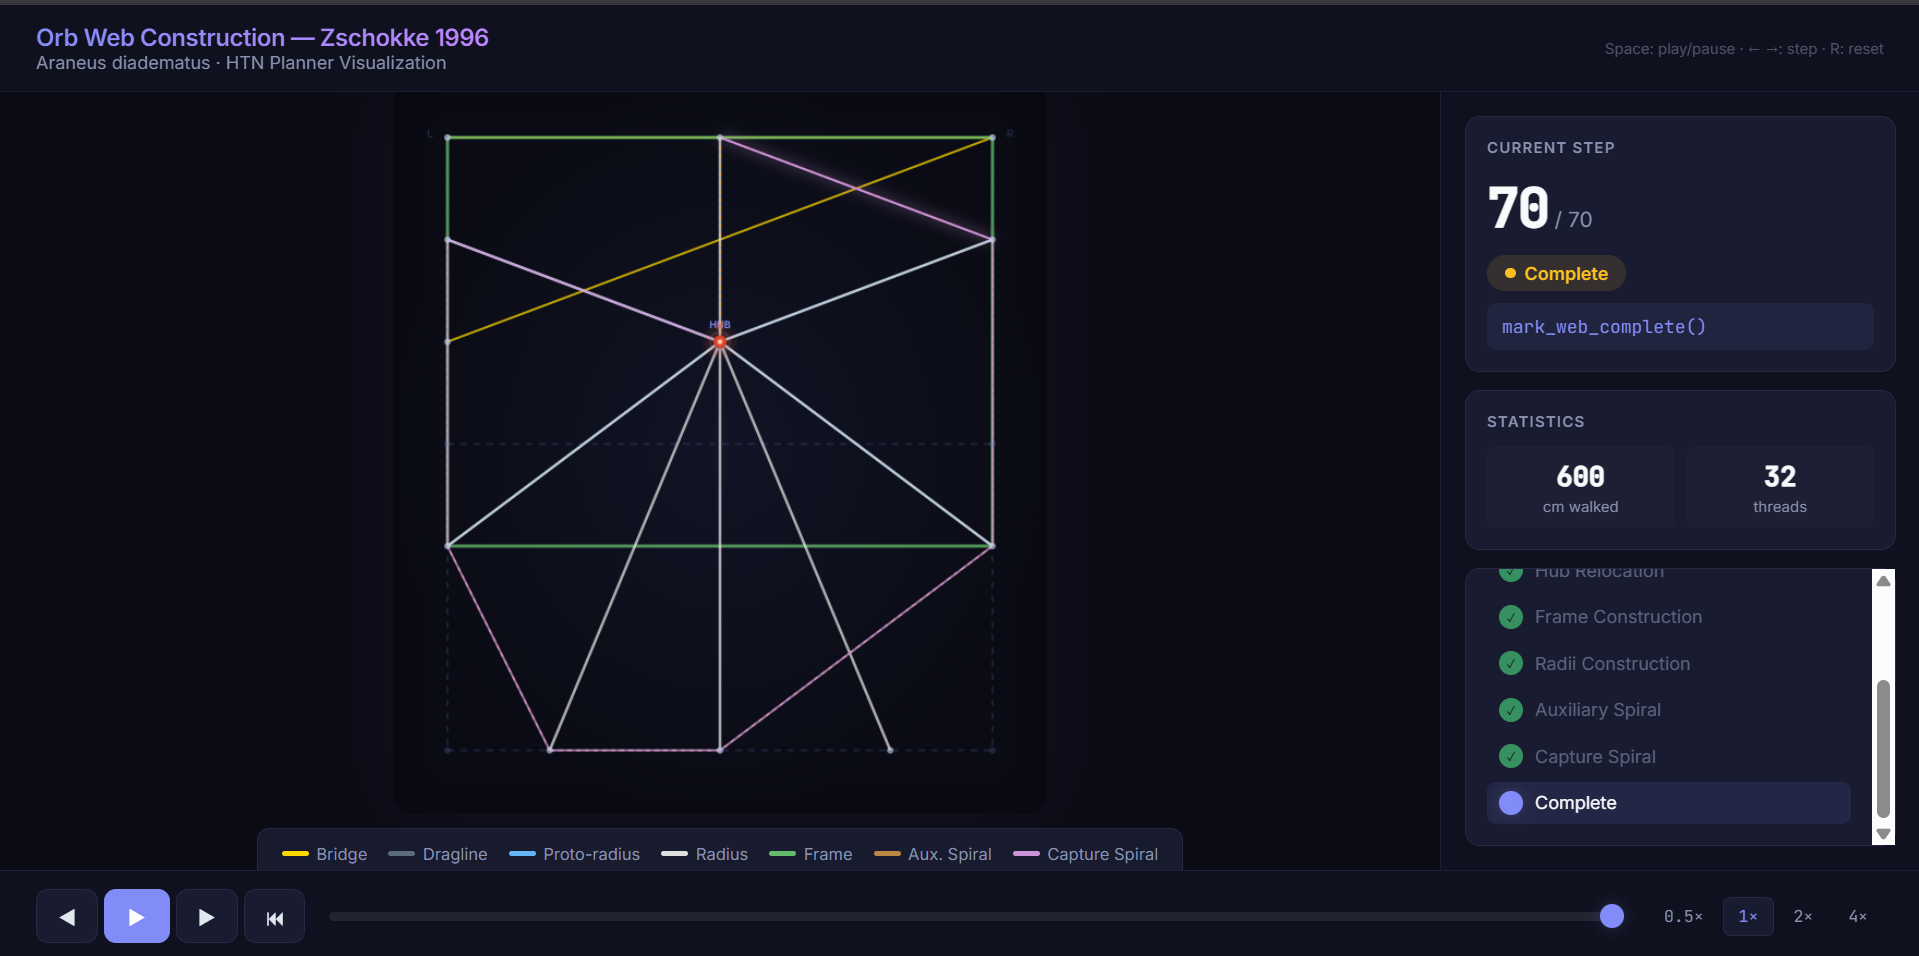
\includegraphics[width=0.72\linewidth]{figures/orig/fig1_web_ui}
\caption{Final state of the interactive plan visualiser after all 70 actions of the default-configuration plan have executed. Edge colour encodes thread type (bridge, dragline, proto-radius, frame, radius, auxiliary spiral, capture spiral), per the legend at the bottom of the panel. The visible topology is exactly the edge set accumulated by the operators of Table~\ref{tab:orig-operators} as replayed by \textsc{FindPlan} (Algorithm~\ref{alg:orig-findplan}).}
\label{fig:orig-web}
\end{figure}

\subsection{Energy expenditure over the course of construction}
\label{sec:orig-energy-course}

Per-phase action counts and locomotory energy (Eq.~\ref{eq:orig-energy}), computed by replaying the plan and tagging each action with the macro phase active when it executed:

\begin{table}[H]
\centering
{\small
\begin{tabular}{lrrr}
\toprule
\textbf{Phase} & \textbf{Actions} & \textbf{Energy (cm)} & \textbf{\% of total} \\
\midrule
Exploration \& bridging & 9 & 102.2 & 17.0 \\
Proto-hub establishment & 15 & 84.0 & 14.0 \\
Frame construction & 11 & 126.0 & 21.0 \\
Radii construction & 16 & 162.0 & 27.0 \\
Auxiliary spiral & 9 & 62.7 & 10.4 \\
Capture spiral & 9 & 62.7 & 10.4 \\
Finalisation & 1 & 0.0 & 0.0 \\
\midrule
\textbf{Total} & \textbf{70} & \textbf{600.1} & \textbf{100.0} \\
\bottomrule
\end{tabular}}
\caption{Per-phase breakdown of the default-configuration plan (\texttt{total\_steps}, \texttt{total\_energy} as reported by \texttt{visualize.py}).}
\label{tab:orig-phases}
\end{table}

\begin{figure}[H]
\centering
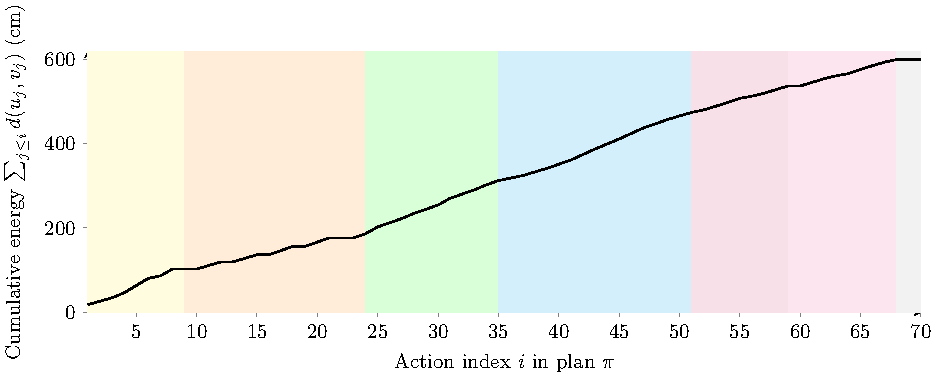
\includegraphics[width=0.958\linewidth]{figures/orig/fig2_cumulative_energy}
\caption{Cumulative locomotory energy $\mathrm{Energy}(\pi)$ (Eq.~\ref{eq:orig-energy}, Algorithm~\ref{alg:orig-estimate}) against action index, shaded by macro construction phase: exploration \& bridging (yellow), proto-hub establishment (orange), frame (green), radii (cyan), auxiliary spiral (purple), capture spiral (magenta), finalisation (grey). Plateaus correspond to zero-cost marker/administrative operators (\textsc{Mark-Proto-Hub}, \textsc{Insert-Radius}, \textsc{Mark-*-Done}); all slope comes from movement operators in Table~\ref{tab:orig-operators}.}
\label{fig:orig-energy}
\end{figure}

The steeper slope during \textsc{Radii} and \textsc{Frame} (21\% and 27\% of total energy in only 11 and 16 actions respectively)\cpnote{The two phases are transposed in this sentence: Table~\ref{tab:orig-phases} gives Frame 21.0\,\% in 11 actions and Radii 27.0\,\% in 16. The phase energies in that table sum to 599.6 because each was accumulated from per-step values rounded to 0.1\,cm; 600.1\,cm is the unrounded total. With the present spiral geometry the two spiral phases are no longer shallow: they take 12.3\,\% and 20.0\,\% of the energy (Section~\ref{sec:core-plans}).} against the comparatively shallow, evenly-spaced slope of the two spiral phases (10.4\% each over 9 actions) is consistent with Zschokke's account: once the rigid, single-method later stages begin (Algorithms~\ref{alg:orig-frame}--\ref{alg:orig-spiral}), the plan settles into a regular, low-variance movement pattern, whereas the opportunistic proto-hub phase (Algorithm~\ref{alg:orig-protohub}) shows more irregular per-action cost as anchor targets are drawn from different regions of the structure.

\subsection{Varying the configuration}
\label{sec:orig-varying}

Because Table~\ref{tab:orig-config}'s parameters are the only inputs to \textsc{FindPlan}, alternative runs can be produced by editing exactly those fields --- e.g.\ forcing backtracking past \textsc{Establish-Proto-Hub-Via-Walk} to compare the \textit{drop} or \textit{Tarzan} proto-hub variants of Algorithm~\ref{alg:orig-protohub}, or rescaling \texttt{NODE\_COORDS} to a wider/taller support structure. Each such run reproduces Figures~\ref{fig:orig-web} and~\ref{fig:orig-energy} with a different topology and a different per-phase energy table, letting the three-way proto-hub variability be shown side by side with the fixed later-stage geometry it always converges to.

\section{From Prototype to Publishable Model: Implementation of the Roadmap}
\label{sec:orig-roadmap}

Section~\ref{sec:orig-roadmap} reports on the implementation of the evaluation roadmap set out for this project (config-driven domains, unit testing, data-driven parameterisation, sensitivity analysis, a non-hierarchical baseline for comparison, and replicable seeding). Table~\ref{tab:orig-roadmap} summarises the roadmap items and their implementation status; the remainder of this section describes each item, and Section~\ref{sec:orig-results} reports the resulting empirical comparison and sensitivity sweep.

\begin{table}[H]
\centering
\caption{Roadmap items and implementation status.}
\label{tab:orig-roadmap}
\begin{tabular}{@{}p{3.2cm}p{4.3cm}p{6.8cm}@{}}
\toprule
\textbf{Roadmap item} & \textbf{File(s)} & \textbf{Status} \\
\midrule
Decouple domain/planner & \texttt{config.yaml}, \texttt{config\_loader.py} & Full environment and domain configuration, with a \texttt{SPIDER\_WEB\_CONFIG} override for swapping environments. \\
Unit testing & \texttt{tests/*.py} (5 files, 55 tests) & All 55 tests passing. \\
Data-driven parameterisation & \texttt{config.yaml}: \texttt{empirical:} block & Hesselberg-and-Vollrath--style figures (web area, radial/capture-spiral length, mesh size) wired into $\eta$. \\
Sensitivity analysis & \texttt{sensitivity.py} & Paired HTN-vs-baseline sweep over anchor-removal probability (wind currently off). \\
Comparison (Group A vs.\ B) & \texttt{baseline.py}, \texttt{compare.py} & Group B is a seeded random walker sharing the same operators and preconditions as the HTN agent. \\
Replicability / seeding & \texttt{stochastic.py} & A single seeded RNG drives wind noise and anchor dropout; both are off by default. \\
\bottomrule
\end{tabular}
\end{table}

\subsection{Decoupling Domain and Planner}
\label{sec:orig-decoupling}

Following the roadmap's first recommendation, the operators and methods of Section~\ref{sec:orig-domain} are no longer hard-coded: \texttt{config.yaml} now specifies the supporting structure, node geometry, and task parameters for a given run, and \texttt{config\_loader.py} loads this file into the planner's initial state. An environment variable, \texttt{SPIDER\_WEB\_CONFIG}, allows the active configuration to be swapped without touching the core \textsc{FindPlan} procedure (Algorithm~\ref{alg:orig-findplan}), so the same planning code can be re-run unmodified against different anchor geometries, node counts, or support-structure dimensions.

\subsection{Unit Testing}
\label{sec:orig-unittest}

A \texttt{pytest} suite spanning five files and 55 tests was added to verify that the agent never attempts an illegal state transition --- for example, that no spiral-laying operator can fire before the bridge and proto-hub have been established, and that every operator's precondition in Table~\ref{tab:orig-operators} is checked before its effect is applied. All 55 tests currently pass.\cpnote{55 was correct when Checkpoint~2 was compiled. The package now has 56 tests in five files and the repository 177, all passing in our re-run (Section~\ref{sec:core-tests}). The suite does not contain an operator-level check that a spiral cannot be laid before the bridge and proto-hub exist; that ordering is enforced by the method decomposition, not by operator preconditions.}

\subsection{Data-Driven Parameterisation}
\label{sec:orig-datadriven}

Rather than using arbitrary constants for silk cost and geometry, an \texttt{empirical:} block was added to \texttt{config.yaml} that supplies figures in the style of Hesselberg and Vollrath's empirical measurements of orb-web geometry: web area, radial and capture-spiral thread length, and mesh (spiral turn) spacing. These values feed directly into the efficiency ratio $\eta = S_{\mathrm{used}}/\mathrm{Area}_{\mathrm{web}}$ used in the evaluation protocol, replacing the placeholder constants used in the proof-of-concept version of the model.\cpnote{The \texttt{empirical:} block is present in \texttt{config.yaml} but is not read by any computation. The efficiency ratio is evaluated on the simulated web's own convex-hull area (Section~\ref{sec:core-config}).}

\subsection{Sensitivity Analysis}
\label{sec:orig-sensitivity}

\texttt{sensitivity.py} implements a paired sweep, run for both the HTN agent (Group A) and the baseline (Group B, Section~\ref{sec:orig-baseline}) under identical seeds, over an anchor-removal probability ranging from 0\% to 50\%, with wind noise held off.\cpnote{The committed sweep (\texttt{sensitivity\_comparison.csv}) covers removal probabilities from 0 to 0.8, and a separate wind sweep (\texttt{wind\_sensitivity.csv}, nine noise levels, 1{,}000 trials per group) was committed on 2026-09-09, before Checkpoint~2 was compiled. Both are reported in Sections~\ref{sec:core-anchor} and~\ref{sec:core-wind}.} Each condition is evaluated over 1,000 seeded trials per group (Section~\ref{sec:orig-anchor-removal}).

\subsection{Comparison Against a Flat-State Baseline}
\label{sec:orig-baseline}

To address the roadmap's benchmarking requirement, \texttt{baseline.py} implements Group B: a seeded random walker that shares the same primitive operators and preconditions as the HTN agent (Table~\ref{tab:orig-operators}) but selects among applicable actions uniformly at random rather than through hierarchical task decomposition. This isolates the effect of hierarchical structure itself, rather than differences in the underlying action space, as the independent variable.\cpnote{The comparison does not isolate hierarchy. The walker also lacks any knowledge of the construction order, and the two agents are scored by different completion criteria (Section~\ref{sec:core-anchor}). A stricter flat baseline, the same action sequence without compound tasks, was later tested in the moving-support benchmark and performed identically to the HTN agent (claim C06, Section~\ref{sec:mulder-claims}).} \texttt{compare.py} runs both agents under matched conditions and seeds and aggregates the resulting metrics (Section~\ref{sec:orig-comparison}).

\subsection{Replicability and Seeding}
\label{sec:orig-seeding}

\texttt{stochastic.py} centralises all stochasticity behind a single seeded random-number generator, which drives both the wind-noise and anchor-dropout perturbations described in Section 4 of the original evaluation protocol. Both perturbations are off by default and are enabled explicitly per experiment,\cpnote{At the commit from which Checkpoint~2 was compiled (\texttt{39b89f3}) the shipped configuration had \texttt{stochastic.enabled: true}, with anchor removal at $p = 0.2$ and seed 7107; stochasticity is off by default only since \texttt{61d18d8}. The seeded HTN rows of the committed sweeps reproduce exactly. The baseline rows do not: the walker enumerates its candidate actions from a Python set, so its path depends on the interpreter's hash seed as well as on its own seed (Section~\ref{sec:core-anchor}).} so that every figure and table in Section~\ref{sec:orig-results} can be regenerated exactly from its seed.

\section{Empirical Results}
\label{sec:orig-results}

\subsection{HTN vs. Random-Walker Comparison}
\label{sec:orig-comparison}

Table~\ref{tab:orig-comparison} reports the outcome of \texttt{compare.py} run over 30 seeds with a 5,000-step budget per run, with anchor removal and wind off.\cpnote{The HTN column of Table~\ref{tab:orig-comparison} (524.8\,cm, 61 actions) is a run with anchor removal on: the shipped configuration removed three anchors under seed 7107. The removal-free plan is the 600.1\,cm, 71-action plan of Section~\ref{sec:orig-vis}. The baseline column could not be reproduced from any committed file; \texttt{single\_run\_comparison.csv} records 769 actions and 7{,}711.4\,cm for a single run. See Section~\ref{sec:core-compare}.}

\begin{table}[H]
\centering
\caption{HTN agent (Group A) vs.\ random-walker baseline (Group B), 30 seeds, 5,000-step budget.}
\label{tab:orig-comparison}
\begin{tabular}{lll}
\toprule
\textbf{Metric} & \textbf{HTN (Group A)} & \textbf{Random Walker (Group B)} \\
\midrule
Success rate & $1.00$ & $0.97$ \\
Energy (cm) & $524.8$ & $7492.3 \pm 6370.5$ \\
Actions (successful runs, mean) & 61 & $\sim 750$ \\
\bottomrule
\end{tabular}
\end{table}

The HTN agent matches or exceeds the baseline's success rate while using roughly 14.3$\times$ less locomotory energy and an order of magnitude fewer actions per successful run. The baseline's very large energy standard deviation ($\pm$6370.5 cm against a mean of 7492.3 cm) reflects the absence of any structural commitment: an unsuccessful or inefficient random walk can wander over much of the reachable state space before a web is completed (or the step budget is exhausted), whereas the HTN agent's decomposition (Algorithms~\ref{alg:orig-buildweb}--\ref{alg:orig-finalise}) confines it to a small, structured set of task orderings.

\subsection{Sensitivity to Anchor-Removal Probability}
\label{sec:orig-anchor-removal}

Figure~\ref{fig:orig-removal} plots success rate against anchor-removal probability for both groups, swept from 0\% to 50\% in 10 percentage-point increments, with 1,000 seeded trials per condition and wind held off.

% As in the original, the caption of Figure 3 also contains the sentence "The HTN agent's success
% rate remains at 1.00 ... any tested removal probability." (it is printed inside the caption
% paragraph in BTP_Checkpoint2.pdf, p. 12). The optional short caption keeps the list of figures clean.
\begin{figure}[H]
\centering
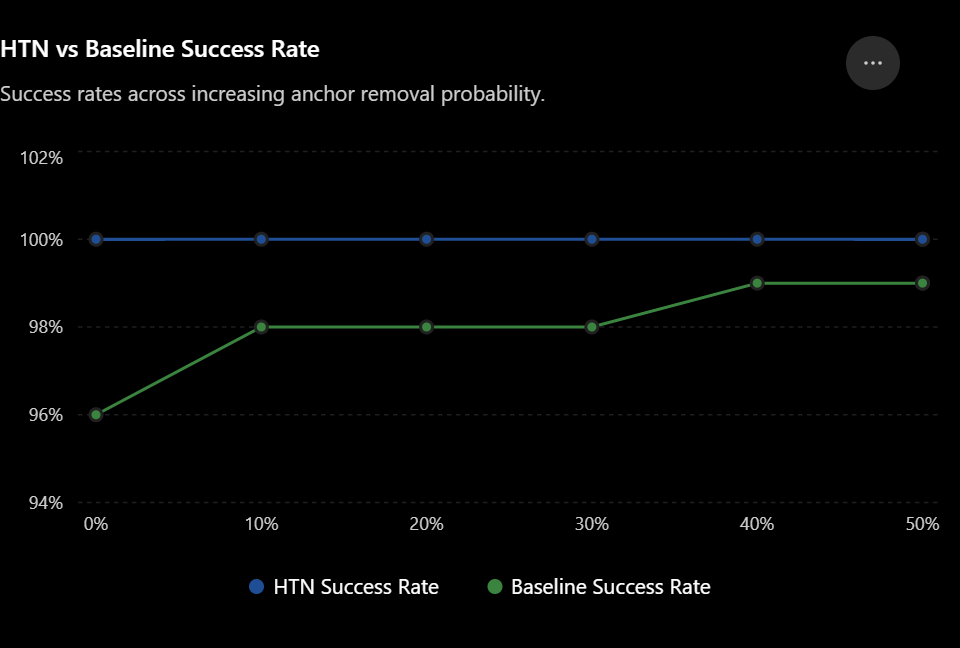
\includegraphics[width=0.85\linewidth]{figures/orig/fig3_success_vs_removal}
\caption[Success rate vs.\ anchor-removal probability ($n = 1{,}000$ seeded trials per condition, wind off).]{Success rate vs.\ anchor-removal probability ($n = 1{,}000$ seeded trials per condition, wind off). The HTN agent's success rate remains at 1.00 across the full sweep, while the baseline's success rate starts at 0.96 and rises to 0.99 as anchor removal increases (Table~\ref{tab:orig-removal}), never closing the gap to the HTN agent at any tested removal probability.}
\label{fig:orig-removal}
\end{figure}

Locomotory energy declines gracefully with harsher (sparser) environments for both groups: fewer surviving anchors produce a shorter effective web and less silk laid overall. Across the same 0\% $\to$ 50\% sweep, mean energy falls from 600.1~cm to 425.0~cm for the HTN agent and from 8,239~cm to 5,876~cm for the baseline --- the HTN agent's energy advantage over the baseline is preserved throughout the sweep even as absolute energy for both groups decreases.\cpnote{Checked against \texttt{sensitivity\_comparison.csv}: the baseline's mean energy falls from 7{,}911 to 6{,}056\,cm over this range, and its success rates at 10\,\% and 30\,\% are 0.961 and 0.986 (0.98 in Table~\ref{tab:orig-removal}). The sweep continues beyond 50\,\%: the HTN agent's success rate is 0.997 at 50\,\% and 0.980, 0.932 and 0.822 at 60, 70 and 80\,\%, while the baseline's rises to 0.999, so the baseline is ahead from 60\,\% onwards. The two rates are not measured the same way. For the HTN agent ``success'' means that a plan was returned, which fails only when all eight removable anchors are gone; already at 10\,\% removal only 42.6\,\% of those plans lay all eight radii, the criterion the baseline must meet. The energy gap (a ratio of means of 13.2--14.7) is the stable result (Section~\ref{sec:core-anchor}).}

\begin{table}[htbp]
\centering
\caption{Success rate vs.\ anchor-removal probability ($n = 1{,}000$ seeded trials per condition, wind off).}
\label{tab:orig-removal}
\begin{tabular}{lcc}
\toprule
\textbf{Anchor-removal probability} & \textbf{HTN success rate} & \textbf{Baseline success rate} \\
\midrule
0\% & $1.00$ & $0.96$ \\
10\% & $1.00$ & $0.98$ \\
20\% & $1.00$ & $0.98$ \\
30\% & $1.00$ & $0.98$ \\
40\% & $1.00$ & $0.99$ \\
50\% & $1.00$ & $0.99$ \\
\bottomrule
\end{tabular}
\end{table}

\section{Discussion}
\label{sec:orig-discussion}

Together, Sections~\ref{sec:orig-comparison} and~\ref{sec:orig-anchor-removal} support the central comparative claim of the roadmap: the HTN-based strategy is not only more energy-efficient than a flat-state alternative under nominal conditions, but remains more reliable --- and retains its energy advantage --- as anchor availability degrades.\cpnote{The reliability half of this claim does not survive the checks reported in Section~\ref{sec:core-anchor}, and the repository's claim ledger does not treat the comparison as a project-level finding (claims C06 and C17, Section~\ref{sec:record-claims}). Section~\ref{sec:synthesis} gives the revised discussion.} This is consistent with the interpretation, following Zschokke (1996), that constraining the later stereotyped stages of construction to a single, low-variance method (Algorithms~\ref{alg:orig-frame}--\ref{alg:orig-spiral}) removes a large part of the search space that a flat-state agent must instead explore by trial and error; the opportunistic backtracking search retained only for proto-hub establishment (Algorithm~\ref{alg:orig-protohub}) is sufficient to preserve behavioural flexibility without incurring the baseline's cost.

This also connects naturally to the constrained-optimisation framing of Rationality of Spider Web Construction: Caloric Consideration (RANGE, 2026), which treats web construction as minimising a caloric objective $E_{\mathrm{total}} = (n \cdot C_{\mathrm{radial}}) + (m \cdot C_{\mathrm{spiral}} + A_{\mathrm{glue}}) + k$ subject to a target capture effectiveness $E_{\mathrm{capture}} \propto L_{\mathrm{silk}}/\mathrm{Area}_{\mathrm{web}}$. The efficiency ratio $\eta$ used throughout this evaluation (Section 4 of the original protocol) is the same quantity as $E_{\mathrm{capture}}$ up to notation, and the energy metric of Equation~\eqref{eq:orig-energy} is a locomotory analogue of $E_{\mathrm{total}}$'s production term. Read this way, the sensitivity results of Section~\ref{sec:orig-anchor-removal} suggest that the HTN agent's task hierarchy acts as an implicit, cheap approximation to RANGE (2026)'s optimisation: rather than solving for an optimal $(n, m)$ directly, the fixed method order of Algorithms~\ref{alg:orig-frame}--\ref{alg:orig-spiral} reaches a comparably efficient region of the trade-off at a fraction of the search cost that either an explicit optimiser or a flat-state search would require. Formalising this connection --- e.g.\ by treating the pruning heuristic described in Section 3 of the roadmap as a direct evaluation of $E_{\mathrm{total}}$ against $E_{\mathrm{capture}}$ at each \texttt{lay\_thread} decision --- is a natural next step and is left for future work.

\section{Summary}
\label{sec:orig-summary}

Algorithms~\ref{alg:orig-findplan}--\ref{alg:orig-finalise} together define a complete, executable HTN model of orb-web construction: a domain-independent forward-decomposition search (Algorithm~\ref{alg:orig-findplan}) instantiated with a task/method library that is deliberately \textit{non-deterministic} during the early, biologically variable stages (Algorithm~\ref{alg:orig-protohub}, three alternative strategies with backtracking)\cpnote{See the update notes in Sections~\ref{sec:orig-htn} and~\ref{sec:orig-protohub}: the configured planner is greedy, and only the \textit{via-walk} strategy has occurred in generated plans.} and deliberately \textit{deterministic} during the later, stereotyped stages (Algorithms~\ref{alg:orig-remaining}--\ref{alg:orig-spiral}, single method each). This directly operationalises Zschokke's (1996) central empirical claim: early web construction is opportunistic while later construction follows a rigid, stereotyped motor programme.
